\documentclass[12pt]{article} % размер шрифта

\usepackage{tikz} % картинки в tikz
\usepackage{microtype} % свешивание пунктуации

\usepackage{array} % для столбцов фиксированной ширины

\usepackage{url} % для вставки ссылок \url{...}

\usepackage{indentfirst} % отступ в первом параграфе

\usepackage{sectsty} % для центрирования названий частей
\allsectionsfont{\centering} % приказываем центрировать все sections

\usepackage{amsthm} % теоремы и доказательства

\theoremstyle{definition} % прямой шрифт в условии теорем
\newtheorem{theorem}{Теорема}[section]


\usepackage{amsmath, amssymb} % куча стандартных математических плюшек

\usepackage[top=2cm, left=1.5cm, right=1.5cm, bottom=2cm]{geometry} % размер текста на странице

\usepackage{lastpage} % чтобы узнать номер последней страницы

\usepackage{enumitem} % дополнительные плюшки для списков
%  например \begin{enumerate}[resume] позволяет продолжить нумерацию в новом списке
\usepackage{caption} % подписи к картинкам без плавающего окружения figure

\usepackage{hyperref} % гиперссылки

\usepackage{verbatim} % побуквенный вывод

\usepackage{fancyhdr} % весёлые колонтитулы
\pagestyle{fancy}
\lhead{Эконометрика, финтех}
\chead{}
\rhead{2018-11-03, встреча 5}
\lfoot{}
\cfoot{}
\rfoot{\thepage/\pageref{LastPage}}
\renewcommand{\headrulewidth}{0.4pt}
\renewcommand{\footrulewidth}{0.4pt}



\usepackage{todonotes} % для вставки в документ заметок о том, что осталось сделать
% \todo{Здесь надо коэффициенты исправить}
% \missingfigure{Здесь будет картина Последний день Помпеи}
% команда \listoftodos — печатает все поставленные \todo'шки

\usepackage{booktabs} % красивые таблицы
% заповеди из документации:
% 1. Не используйте вертикальные линии
% 2. Не используйте двойные линии
% 3. Единицы измерения помещайте в шапку таблицы
% 4. Не сокращайте .1 вместо 0.1
% 5. Повторяющееся значение повторяйте, а не говорите "то же"

\usepackage{fontspec} % поддержка разных шрифтов
\usepackage{polyglossia} % поддержка разных языков

\setmainlanguage{russian}
\setotherlanguages{english}

\setmainfont{Linux Libertine O} % выбираем шрифт
% если Linux Libertine не установлен, то
% можно также попробовать Helvetica, Arial, Cambria и т.Д.

% чтобы использовать шрифт \Linux Libertine на личном компе,
% его надо предварительно скачать по ссылке
% http://www.\Linuxlibertine.org/index.php?id=91&L=1

% на сервисах типа sharelatex.com этот шрифт есть :)

\newfontfamily{\cyrillicfonttt}{Linux Libertine O}
% пояснение зачем нужно шаманство с \newfontfamily
% http://tex.stackexchange.com/questions/91507/

\AddEnumerateCounter{\asbuk}{\russian@alph}{щ} % для списков с русскими буквами
\setlist[enumerate, 2]{label=\asbuk*),ref=\asbuk*} % списки уровня 2 будут буквами а) б) ...

%% эконометрические и вероятностные сокращения
\DeclareMathOperator{\Cov}{Cov}
\DeclareMathOperator{\sCov}{sCov}
\DeclareMathOperator{\sVar}{sVar}
\DeclareMathOperator{\sCorr}{sCorr}
\DeclareMathOperator{\Corr}{Corr}
\DeclareMathOperator{\Var}{Var}
\DeclareMathOperator{\E}{E}
\DeclareMathOperator{\tr}{trace}
\DeclareMathOperator{\trace}{trace}
\DeclareMathOperator{\Lin}{Lin}
\DeclareMathOperator{\Linp}{Lin^{\perp}}


\def \hb{\hat{\beta}}
\def \hs{\hat{\sigma}}
\def \htheta{\hat{\theta}}
\def \s{\sigma}
\def \hy{\hat{y}}
\def \hY{\hat{Y}}
\def \v1{\vec{1}}
\def \e{\varepsilon}
\def \he{\hat{\e}}
\def \z{z}
\def \hVar{\widehat{\Var}}
\def \hCorr{\widehat{\Corr}}
\def \hCov{\widehat{\Cov}}
\def \cN{\mathcal{N}}
\def \RR{\mathbb{R}}

\makeatletter
\def\MT@warn@unknown{}
\makeatother




\begin{document}

Конспектировал: Ярослав Романов.

\section{Дифференциальные формы}

\begin{flushright}
  \textit{Хорошо было бы работать не с плотностями,\\а с дифференциальными формами}.
\end{flushright}

\vspace{\baselineskip}

% картинка
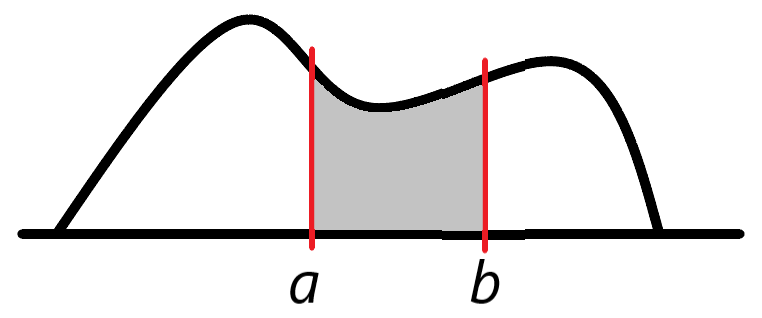
\includegraphics[width=5cm]{images/05_pic1.png}

Идея: если хотим найти вероятность, что случайная величина $\omega$ примет значение от $a$ до $b$, мы можем посчитать интеграл:

\[
    P(\omega \in [a, b]) = \int \limits_{a}^{b} f(t)dt
\]

Если при этом, мы хотим произвести замену переменной $\omega = Z^3$ и найти функцию плотности распределения $Z^3$, то просто подставить $z^3$ в  формулу функции распределения для $\omega$ будет некорректно.

И тут нам на помощь приходит дифференциальная форма. Идея дифференциальной формы "на пальцах" заключается в том, что нам необходимо следить не за высотой, а за прямоугольно областью (в случае одномерной случайной величины):

% картинка
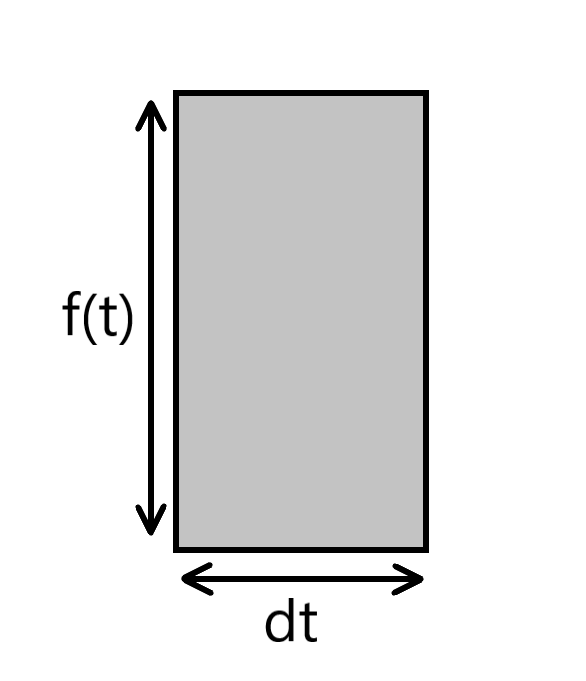
\includegraphics[width=3cm]{images/05_pic2.png}

Значение фукции плотности $f(t)$ в данном случае отвечает за высоту, а приращение аргумента $dt$ — за ширину нашего прямоугольника.\\

\textit{Пример}:\\
Пусть имеется случайная величина $\omega \sim U[0,1]$, $Z = \omega^3$. Требуется найти функцию плотности распределения $f_Z(t)$.
Дифференциальная форма $\omega$ есть:
\[
    \begin{cases}
        1da &\text{при $a$ \in [0,1]}\\
        0da &\text{при $a$ \in [0,1]}
    \end{cases}
\]

Произведем замену $\omega = Z^{\frac{1}{3}}$ и, соответственно, $\omega = z^{\frac{1}{3}}$.
Тогда для $Z$ получим следующую дифференциальную форму:
$1dz^{\frac{1}{3}} = \frac{1}{3}z^{-\frac{2}{3}}dz$,
в которой часть перед дифференциалом и будет искомой функцией распределения:
$f_Z(z) = \frac{1}{3}z^{-\frac{2}{3}}$.

Как будет работать данный прием в случае с совместным распределением случайных величин $f(a,b)$? Для того, чтобы удобнее оперировать дифференциальными формами в этом случае, мы будем использовать так называемое внешнее умножение, обозначаемое как $\wedge$ ("птичка"):
$f(a,b) \rightarrow f(a,b)da \wedge db$
Отметим правила внешнего умножения, которыми нам помогут в дальнейших расчетах:
\subitem {Правило 1: $da \wedge da = 0$}
\subitem {Правило 2: $da \wedge db = - db \wedge da$}.\\


\textit{Упражнение}:\\
Пусть есть пара случайных величин $Y$ и $\omega$ и задана их плотность совместного распределения:
\[
    f(y, \omega)=
    \begin{cases}
        4 y \omega &\text{$y$, \omega \in [0,1]}\\
        0 &\text{иначе}
    \end{cases}
\]
Введем новые случайные величины $R$ и $S$ и определим соотношение с $Y$ и $\omega$:
\[
    R = Y + \omega^3,
\]
\[
    S = 2 Y + 3\omega^3
\]
Требуется найти функцию плотности распределения $R$ и $S$ $f_{R,S}(r,s)$
Итак,
\[
    P(Y \in [y; y + dy], \omega \in [\omega; \omega + d\omega]) \sim 4 y \omega dy \wedge d\omega
\]
Сделаем замену
\[
    \begin{cases}
        r = y + \omega^3\\
        s = 2 y + 3 \omega^3
    \end{cases}
\]
тогда
\[
    \begin{cases}
        y = 3 r - s\\
        \omega = (s - 2 r)^{\frac{1}{3}}
    \end{cases}
\]
Из этого следует, что:
\begin{eqnarray*}
    P(Y \in [y; y + dy], \omega \in [\omega; \omega + d\omega]) =\\
    = 4(3 r - s)(s - 2 r)^{\frac{1}{3}}(3 dr - ds) \wedge (\frac{1}{3} (s - 2 r)^{-\frac{2}{3}} (ds - 2 dr)) =\\
    = 4(3 r - s)(s - 2 r)^{-\frac{1}{3}}(3 dr - ds) \wedge (ds -2 dr) =\\
    = 4(3 r - s)(s - 2 r)^{-\frac{1}{3}}(3 dr \wedge ds + 2 ds \wedge dr) =\\
    = \frac{4}{3}(3 r - s)(s - 2 r)^{-\frac{1}{3}} dr \wedge ds
\end{eqnarray*}

Таким образом, функция плотности совместного распределения $R$ и $S$ — это все, что находится перед дифференциалами:
\[
    f_{R,S}(r,s) = \frac{4}{3}(3 r - s)(s - 2 r)^{\frac{1}{3}}
\]



\textit{Упражнение}:\\
Пусть даны случайные независимые величины $Z_1, Z_2, \ldots, Z_{10}$ из равномерного распределения $U[0,1]$\\
Упорядочим случайные величины по возрастанию их значений и переобозначим как $Y_1, Y_2, \ldots, Y_{10}$\\
% картинка
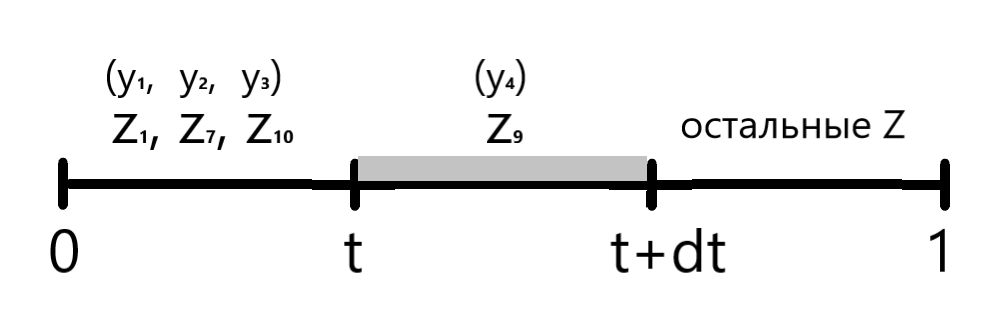
\includegraphics[width=7cm]{images/05_pic4.png}

Требуется найти функцию плотности распределения четвертой по величини случайной величины $f_{Y_4}(t)$.\\
Воспользуемся дифференциальными формами и попробуем найти $f_{Y_4}(t) dt + o(dt)$
\begin{eqnarray*}
    f_{Y_4}(t) dt + o(dt) =\\
    P(Y_4 \in [t; t + dt]) =\\
    t^3 (1 - t)^6 10  C_9^3 \frac{dt}{1} + o(dt)
\end{eqnarray*}

Как мы уже знаем, функция плотности распределения $Y_4$ — это все, что находится перед дифференциалами:
\[
    f_{Y_4}(t) = 10 C_9^3 t^3 (1 - t)^6
\]


\section{Распределения}
Мы разобрались с удобным способом работы функциями распределений случайных величин. Теперь, пользуясь этим знанием, перейдем ближе к делу — определим некоторые распределения случайных величин
\subsection{Экспоненциальное распределение}
Аксиома: вероятность того, что ученик, ищущий просветления, достигнет его за малый отрезок времени, пропорциональна длине этого отрезка.
Случайная величина $Y$ обозначает время от начала познания до просветления
Хотим найти: функцию плотности распределения $f(Y)$

%картинка
%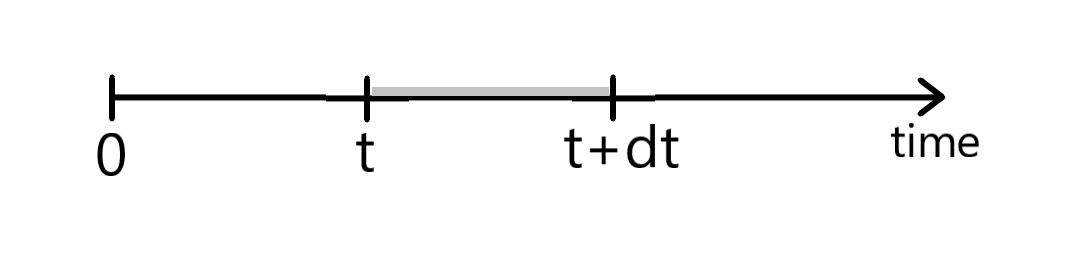
\includegraphics[width=6cm]{images/05_pic3.png}

\[
    P(Y \geq t + dt) = P(Y \geq t)(1 - \lambda dt - o(dt))
\]
Обозначим $P(Y \geq t)$ за $h_t$, тогда:
\begin{eqnarray*}
    h_{t + dt} = h_t - \lambda h_t dt - h_t o(dt),\\
    h_{t + dt} - h_t = - \lambda h_t dt + o(dt),\\
    \frac{h_{t + dt} - h_t}{dt} = - \lambda h_t + \frac{o(dt)}{dt}
\end{eqnarray*}
тогда
\[
    h_t = \exp(- \lambda t)
\]
а искомая функция плотности распределения после взятия производной вероятности равна:
\[
    f(y) = \lambda \exp(- \lambda t)
\]


\subsection{Гамма и бета распределения}
Аксиома: Тётя-Мотя печет блинчики: внуку $a$ штук и на продажу $b$ штук. Оборудование Тёти-Моти в процессе приготовления переводит блин из сырого состояния в готовое моментально. Вероятность испечь очередной блинчик за малый отрезок времени пропорциональна длине этого отрезка времени.
Случайная величина $S$ обозначает общее время выпечки всех блинчиков. Следовательно, $S$ принимает значение от нуля до бесконечности
Случайная величина $R$ равна доле времени, потраченного на выпечку блинчиков для внука. Следовательно, $R$ принимает значения от нуля до единицы.
В нашем контесте $S$ распределена по гамма-закону, а $R$ — по бета-закону
Хотим найти для $R$ и $S$ функции плотности их распределений $f(r)$ и $f(s)$
Заметим, что $R$ и $S$ независимы по смыслу, поэтому
$f(r,s) = f(r) f(s)$\\

\textit{Случай 1}:\\
Для начала рассмотрим простой частный случай, при котором $a = 1$ и $b = 1$.\\
Требуется найти $f(r), f(s)$.\\
Пусть $Y_1$ и $Y_2$ — время на выпечку первого и второго блина соответственно.\\
Мы уже знаем функцию плотности экспоненциально распределенной величины, поэтому:
\[
    f(y_1) = \lambda \exp(- \lambda y_1)
\]
\[
    f(y_2) = \lambda \exp(- \lambda y_2)
\]
Тогда:
\[
    P(Y_1 \in [y_1; y_1 + dy], Y_2 \in [y_2; y_2 + dy]) \sim \lambda \exp(- \lambda y_1) \lambda \exp(- \lambda y_2) dy_1 \wedge dy_2
\]
Также по условию задачи:
\[
    S = Y_1 + Y_2
\]
и
\[
    R = \frac{Y_1}{Y_1 + Y_2}
\]
Или иначе:
\[
    Y_1 = R S
\]
\[
    Y_2 = S - Y_1 = S - R S
\]
Подставим полученное в формулу вероятности
\begin{eqnarray*}
    \lambda \exp(- \lambda r s) \lambda \exp(- \lambda (s - rs)) d(r s) \wedge d(s - r s) =\\
    = \lambda^2 \exp(- \lambda s) d(r s) \wedge ds =\\
    = \lambda^2 \exp(- \lambda s) (s dr + r ds) \wedge ds =\\
    = \lambda^2 \exp(- \lambda s) s dr \wedge ds
\end{eqnarray*}
Следовательно,
\[
    f(r, s) = \lambda^2 \exp(- \lambda s) s \cdot 1
\]
\[
    f(s) =
    \begin{cases}
        \lambda^2 \exp(- \lambda s) s &\text{при $s > 0$}\\
        0 &\text{иначе}
    \end{cases}
\]
\[
    f(r) =
    \begin{cases}
        1 &\text{при $r \in [0,1]$}\\
        0 &\text{иначе}
    \end{cases}
\]

\textit{Случай 2}:\\
Пусть теперь $a = 2$, а $b = 1$\\
Требуется найти $f(r), f(s_3)$.\\
Время на два блинчика (или время на блины внуку, соответственно):
\[
    S_2 = Y_1 + Y_2
\]
а время на все три блинчика:
\[
    S_3 = S_2 + Y_3
\]
и
\[
    R = \frac{Y_1}{S_2 + Y_3}
\]
Тогда:
\[
    S_2 = R S_3
\]
\[
    Y_3 = S_3 - R S_3
\]
Посчитаем в сторонке выражение с "птичками":
\begin{eqnarray*}
    ds_2 \wedge dy_3 =\\
    = d(r s_3) \wedge (ds_3 - d(r s_3) =\\
    = d(r s_3) \wedge ds_3 =\\
    = s_3 dr \wedge ds_3
\end{eqnarray*}
Посчитаем искомую вероятность:
\begin{eqnarray*}
    P(S_2 \in [s_2; s_2 + ds_2], Y_3 \in [y_3, y_3 + dy_3]) \sim\\
    \sim (\lambda^2 \exp(- \lambda s_2) s_2) \lambda \exp(- \lambda y_3) ds_2 \wedge dy_3 =\\
    = \lambda^3 \exp(- \lambda s_3) r s_3^2 dr \wedge ds_3
\end{eqnarray*}
Следовательно,
\[
    f(r, s_3) = \lambda^3 \exp(- \lambda s_3) r s_3^2 = (\frac{1}{2} \lambda^3 \exp(- \lambda s_3) s_3^2) (2 r)
\]
\[
    f(s_3) =
    \begin{cases}
        \frac{1}{2} \lambda^3 \exp(- \lambda s_3) s_3^2 &\text{при $s_3 > 0$}\\
        0 &\text{иначе}
    \end{cases}
\]
\[
    f(r) =
    \begin{cases}
        2 r &\text{при $r \in [0,1]$}\\
        0 &\text{иначе}
    \end{cases}
\]
Используя метод индукции и результаты, полученные ранее в частных случаях, определим математическое ожидание для изучаемых распределений.\\
Случайная величина $S_k$, имеющая гамма-распределение с параметрами $\lambda$ и $k$, будет иметь функцию плотности распределения, пропорциональную некоторому выражению:
\[
    f(s_k) \propto \lambda^k \exp(- \lambda s_k) s_k^{k - 1}
\]
Тогда математическое ожидание величины $S_k$:
\[
    E(S_k) = \int \limits_{0}^{\infty} s_k f(s_k) ds_k
\]
либо без знания функции плотности:
\[
    E(S_k) = K E(Y_1) = K \int \limits_{0}^{\infty} y_1 f(y_1) dy_1
\]
либо еще круче, когда даже для $Y_1$ нам не известна функция плотности:
\[
    E(Y_1) = \mu
\]
и вероятность того, что блин испечется в отрезке времени $[0, dt]$ равна $p = \lambda dt + o(dt)$
\begin{eqnarray*}
    \mu = (1 - \lambda dt - o(dt)) (dt + \mu) + (\lambda dt + o(dt)) dt =\\
    = dt - \lambda(dt)^2 + o(dt)dt + \mu - \lambda \mu dt + d(dt) \mu + \lambda dt^2 + o(dt)
\end{eqnarray*}
\[
    dt = \lambda \mu dt + o(dt)\\
\]
\[
    \frac{dt}{dt} = \frac{\lambda \mu dt}{dt} + \frac{o(dt)}{dt}, dt \rightarrow 0\\
\]
\[
    1 = \lambda \mu\\
\]
\[
    \mu = \frac{1}{\lambda}
\]

\textit{Случай 3}:\\
Еще обобщим ситуацию. Пусть теперь общее количество блинчиков $k = 3$\\
Требуется найти $f(r_1), f(r_2), f(s_3)$.\\
Время на все три блинчика:
\[
    S_3 = Y_1 + Y_2 + Y_3
\]
и
\[
    R_1 = \frac{Y_1}{Y_1 + Y_2}
\]
\[
    R_2 = \frac{Y_1 + Y_2}{Y_1 + Y_2 + Y_3}
\]
Тогда:
\[
    y_1 = r_1 r_2 s_3
\]
\[
    y_2 = r_2 s_3 - r_1 r_2 s_3
\]
\[
    y_3 = s_3 - r_2 s_3
\]
Запишем дифференциальные формы для $Y_1, Y_2, Y_3$.\\
Но для начала посчитаем в сторонке выражение с "птичками":
\begin{eqnarray*}
    dy_1 \wedge dy_2 \wedge dy_3 =\\
    = d(r_1 r_2 s_3) \wedge d(r_2 s_3 - r_1 r_2 s_3) \wedge d(s_3 - r_2 s_3) =\\
    = d(r_1 r_2 s_3) \wedge d(r_2 s_3) \wedge d(s_3 - r_2 s_3) =\\
    = d(r_1 r_2 s_3) \wedge d(r_2 s_3) \wedge d(s_3) =\\
    = (r_2 s_3 d(r_1) + r_1 d(r_2 s_3)) \wedge d(r_2 s_3) \wedge d(s_3) =\\
    = r_2 s_3 s_3 dr_1 \wedge dr_2 \wedge ds_3
\end{eqnarray*}
Тогда по знакомой нам схеме:
\begin{eqnarray*}
    P(Y_1 \in [y_1, y_1 + dy_1], Y_2 \in [y_2, y_2 + dy_2], Y_3 \in [y_3, y_3 + dy_3]) =\\
    = \lambda \exp(- \lambda y_1) \lambda \exp(- \lambda y_2) \lambda \exp(- \lambda y_3) d(y_1) \wedge d(y_2) \wedge d(y_3) =\\
    = \lambda^3 \exp(- \lambda s_3) r_2 s_3^2 dr_1 \wedge dr_2 \wedge ds_3
\end{eqnarray*}
Следовательно,
\[
    f(r_1, r_2, s_3) = 1 \cdot 2 r_2 \cdot \frac{1}{2} \lambda^3 \exp(- \lambda s_3) s_3^2
\]
И в силу независимости случайных величин $R_1, R_2, S_3$
\[
    f(s_3) =
    \begin{cases}
        \frac{1}{2} \lambda^3 \exp(- \lambda s_3) s_3^2 &\text{при $s_3 > 0$}\\
        0 &\text{иначе}
    \end{cases}
\]
\[
    f(r_1) =
    \begin{cases}
        1 &\text{при $r_1 \in [0,1]$}\\
        0 &\text{иначе}
    \end{cases}
\]
\[
    f(r_2) =
    \begin{cases}
        2 r_2 &\text{при $r_2 \in [0,1]$}\\
        0 &\text{иначе}
    \end{cases}
\]






\end{document}
